\section{湯気のシミュレーション}

\subsection{湯気の発生原理}

湯気の発生と消滅のプロセスの詳細を記載する。
ここでは常温の空気中に存在する液体の水の水面上から湯気が発生している状態を対象とする。
この時、水温は空気の温度よりも高いが沸騰はしていない状態とする。

まず水が水面上から液体が気体へ蒸発し、蒸発した水蒸気は分子拡散により周囲へ拡散する。
同時に水の温度は空気よりも高いため温度勾配により熱拡散が起こり熱が水から空気へ移動する。
空気の温度が上昇すると空気の密度が周囲の空気より低くなることにより浮力が発生する。
浮力により空気へ上方向の力が働き、対流が発生する。
この対流により空気に含まれる水蒸気、熱が移動する。
空気中に含まれる水蒸気量が飽和水蒸気量を超えた場合に凝結することで水滴が発生する。
凝結は大気中の細かい塵を核として行われる。
この水滴の粒子に対して光が当たった際に散乱が起こり白く見えることで湯気として認識される。
凝結により発生する水滴の粒子は光の波長と同程度、もしくは少し大きめの大きさとなりミー散乱という現象が発生する。
ミー散乱は粒子のサイズが大きくなるにつれて前方の指向性が高くなり側方、後方への散乱は弱くなる。
空気中に含まれる水蒸気量が飽和水蒸気量を下回った場合、水滴が空気中に蒸発し湯気が消滅する。

\subsection{シミュレーションモデル}

湯気の速度$\upsilon=(u,v,w)$は非粘性、非圧縮のオイラーの運動方程式(\ref{continuity},\ref{euler})によって与えられる。


\begin{equation}
\label{continuity}
\nabla \cdot \upsilon = 0
\end{equation}
\begin{equation}
\label{euler}
\frac{\partial \upsilon}{\partial t} = -(\upsilon \cdot \nabla)\upsilon - \nabla p + B + f
\end{equation}

$B$は浮力、$f$は風などによる外力を表す。浮力$B$は式(\ref{buoyancy})で定義する。
\begin{equation}
\label{buoyancy}
B=(k_{b}\Delta{T}-gq_{c})z
\end{equation}
$k_{b}$は浮力の係数、$g$は重力の係数、$q_{c}$は湯気の濃度、$z$は上方向のベクトルである。
湯気が発生する底面周辺のように温度変化が大きい場合、近似による誤差が大きくなる。
このため周辺の温度の差分から上向きの浮力の計算を行う。

湯気の密度$q_{c}$と水蒸気$q_{v}$の密度は次式で定義する。
\begin{equation}
\label{steam}
\frac{\partial q_{c}}{\partial t} = -(\upsilon \cdot \nabla)q_{c} + C_{c}
\end{equation}
\begin{equation}
\label{vapor}
\frac{\partial q_{v}}{\partial t} = D_{v}\nabla^2q_{v}-(\upsilon \cdot \nabla)q_{v} - C_{c} + S_{v}
\end{equation}
$D_{v}$は水蒸気の分子拡散係数、$C_{c}$は相転移によって発生する湯気の量、$S_{v}$は水蒸気源から水蒸気の供給量である。

分子拡散係数$D_{v}$は次式で表され。これはアインシュタイン・ストークスの式より温度に依存する。
\begin{equation}
\label{diffusion}
D_{v}=D_{0}T
\end{equation}
ここで$D_{0}$は分子拡散係数を決定するためのパラメータである。

相転移によって発生する湯気の量$C_{c}$は次式で表される。
\begin{equation}
\label{transition}
C_{c} = \alpha(q_{v}-q_{s})
\end{equation}
ここで$\alpha$は相転移率である。

$q_{s}$は飽和水蒸気密度を表し、次式で与えられる。	
\begin{equation}
\label{saturation}
q_{s} = \min\left(S_{a} \exp\left(\frac{-S_{b}}{T+S_{c}}\right),q_{v}+q_{c}\right)
\end{equation}
ここで$S_{a},S_{b},S_{c}$は飽和水蒸気密度を決定するためのパラメータである。

温度$T$は以下のように表される。
\begin{equation}
\label{temperature}
\frac{\partial T}{\partial t} = D_{t}\nabla^2T- (\upsilon \cdot \nabla)T +  QC_{c} + S_{T}
\end{equation}
ここで$D_{t}$は熱拡散率、$Q$は潜熱係数を表す。
右辺第一項は熱拡散、第二項は熱対流、第三項は相転移による潜熱、第四項は外部の熱源からの熱量を表す。
水蒸気源と熱源は空間の底面から発生し、発生量の分布はユーザにより定義する。

\subsection{実装}
シミュレーション空間は$N_{x} \times N_{y} \times N_{z}$の格子に分割し各格子点に温度$T$,水蒸気密度$q_{v}$,湯気の密度$q_{c}$を割り付ける。
初期状態として水蒸気源と熱源が存在する部分には水蒸気密度と温度の固定値を割り付けられる。
\begin{figure}
	\begin{center}
		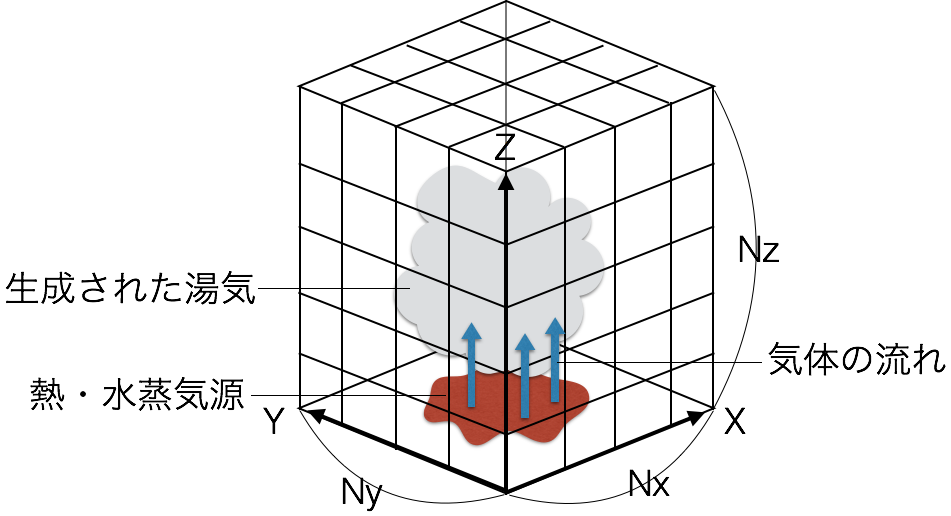
\includegraphics[width=100mm]{simulation.png}
		\caption{湯気のシミュレーション空間}
		\label{simulation}
	\end{center}
\end{figure}
全体の処理の流れとしては温度による浮力の計算、水蒸気と温度の拡散の計算、水蒸気と温度および湯気の移流の計算、圧力と質量保存則の効果の計算を繰り返す。
浮力は計算対象の格子の温度と周囲の格子の温度の差から計算を行う。
水蒸気と温度の拡散の計算は拡散方程式の数値解法を用いる。
水蒸気と温度および湯気の移流の計算、圧力と質量保存則の効果の計算には\ref{smoke}章に記載したFedkiwら\cite{Fedkiw2001}の手法を用いる。



